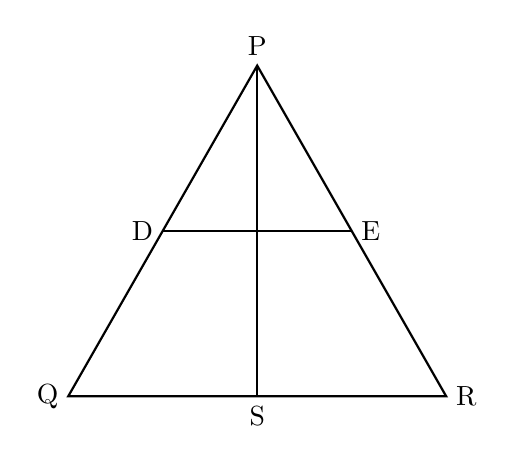
\begin{tikzpicture}[scale=1.2]

    % --- Define Coordinates ---
    % S is the midpoint of the base
    \coordinate (S) at (0,0);
    
    % Q is the bottom-left vertex
    \coordinate (Q) at (-2,0);
    
    % R is the bottom-right vertex
    \coordinate (R) at (2,0);
    
    % P is the top apex vertex
    \coordinate (P) at (0,3.5);
    
    % D lies on segment PQ (midpoint visually)
    \coordinate (D) at (-1, 1.75);
    
    % E lies on segment PR (midpoint visually)
    \coordinate (E) at (1, 1.75);

    % --- Draw Lines and Segments ---
    
    % Draw the main triangle PQR
    \draw[thick] (P) -- (Q) -- (R) -- cycle;

    % Draw the vertical segment PS (Altitude/Median)
    \draw[thick] (P) -- (S);

    % Draw the horizontal segment DE
    \draw[thick] (D) -- (E);

    % --- Place Labels ---
    
    % Label P at the top
    \node[above] at (P) {P};
    
    % Label Q at the bottom-left
    \node[left] at (Q) {Q};
    
    % Label R at the bottom-right
    \node[right] at (R) {R};
    
    % Label S at the bottom center
    \node[below] at (S) {S};
    
    % Label D to the left of the intersection
    \node[left] at (D) {D};
    
    % Label E to the right of the intersection
    \node[right] at (E) {E};

\end{tikzpicture}